\section{CARA: Coherent Adaptive Reasoning Agents}
\label{sec:cara}
As described earlier, CARA (Coherent Adaptive Reasoning Agents) implements the \emph{reflect} operation. Given
the long-term memory bank built and
maintained by TEMPR,
CARA turns retrieved facts and observations into preference-conditioned reasoning and a layer of explicitly stored opinions that can change over time.
CARA treats an agent's \emph{behavioral profile} as a first-class part of the system configuration rather than as a one-off prompt decoration. Each memory bank is associated with a configurable disposition profile (skepticism, literalism, empathy) and a concise background description, and CARA uses this profile when forming and updating opinions over the world and experience networks.

Concretely, CARA provides four key capabilities: disposition-profile integration, \our memory integration, opinion formation and reinforcement, and background merging with conflict resolution.

\subsection{Motivation}

To motivate CARA, consider two configurations of the same agent discussing remote work. 

In the first configuration, given a behavioral profile with low skepticism ($S = 1$), flexible interpretation ($L = 2$), and high empathy ($E = 5$), an agent might form the opinion: ``Remote work enables creative flexibility and spontaneous innovation.'' 

In the second configuration, given high skepticism ($S = 5$), highly literal interpretation ($L = 5$), and low empathy ($E = 1$), the same facts might instead yield: ``Remote work lacks the structure and accountability needed for consistent performance.''

Both configurations access identical factual information from the \our memory bank, but their behavioral profiles bias how they weight different aspects (viz. flexibility vs.\ structure) and what conclusions they draw. CARA provides a mechanism to specify such behavioral profiles and to systematically shape opinion formation and updating as a function of these configuration choices.

\subsection{Preference Model}

CARA first defines a preference space that can be parameterized and verbalized for prompting.

\subsubsection{Disposition Parameters}

We use a three-dimensional disposition space as an interpretable set of ordered preference dimensions. Let $\Theta = (S, L, E, \beta)$ denote a behavioral profile where:
\begin{align}
S &\in \{1,\ldots,5\} \quad \text{(Skepticism; 1 = trusting, 5 = skeptical)} \\
L &\in \{1,\ldots,5\} \quad \text{(Literalism;  1 = flexible, 5 = literal)} \\
E &\in \{1,\ldots,5\} \quad \text{(Empathy; 1 = detached, 5 = empathetic)} \\
\beta &\in [0,1] \quad \text{(Bias strength: controls influence of preferences)}
\end{align}

The bias strength parameter $\beta$ controls how strongly the behavioral profile should shape opinion formation. When $\beta = 0$, reasoning is primarily fact-based. When $\beta = 0.5$, there is moderate influence from the behavioral profile. When $\beta = 1$, there is strong preference-conditioned behavior.

\paragraph{Rationale for using Disposition Parameters.}

We adopt these dimensions because they offer a compact, interpretable parameterization of reasoning style (trusting vs.\ skeptical, flexible vs.\ literal, detached vs.\ empathetic), intuitive axes that can be verbalized in prompts (e.g., ``skeptical but highly empathetic''), and a simple interface for users configuring different agent styles.

\paragraph{Intended Effects on Reasoning.}

CARA uses the behavioral profile to modulate prompts so that different configurations encourage different emphases when forming opinions. The mapping from preference values to reasoning behavior is achieved through natural language verbalization in system prompts. Higher Skepticism encourages more cautious evaluation of claims, greater emphasis on evidence quality, and reluctance to accept unsupported statements; lower Skepticism encourages more trusting and exploratory behavior. Similarly, higher Literalism encourages closer attention to exact wording and explicit instructions; lower Literalism encourages reading between the lines, inferring implicit goals, and using abstraction. Finally, higher Empathy encourages taking emotional context and interpersonal impact into account, using more supportive and face-saving language; lower Empathy encourages more blunt, task-first communication.

\subsection{Bank Profile Structure}

Each memory bank has an associated profile that encodes the agent's identity and disposition configuration in a form suitable for prompting and reasoning. Formally, a bank profile is a tuple:
\begin{equation}
P = (n, \Theta, h)
\end{equation}
where $n$ is the agent's name, $\Theta = (S, L, E, \beta)$ is the behavioral profile, and $h$ is a short background description written in the first person.

\subsubsection{Preference Description Generation}

The numeric behavioral profile $\Theta$ is verbalized into natural language so it can be injected into system messages. Let $\phi: \Theta \rightarrow \text{String}$ be a verbalization function that converts numeric values to descriptive text. For example:
\begin{equation}
\phi(\Theta) = \text{``You are generally trusting, interpret language flexibly, and are highly empathetic ..."}
\end{equation}
This verbalization connects the numeric preference configuration to the LLM's behavior by providing an explicit description of how the agent is intended to reason and communicate.

\subsection{Opinion Network and Opinion Formation}

\subsubsection{Opinion Structure}

Opinions are stored in the opinion network $\mathcal{O}$, separate from world and bank facts. Each opinion is a self-contained memory that records both the judgment and the context in which it was formed. Formally, an opinion is a tuple:
\begin{equation}
o = (t, c, \tau, b, \mathcal{E})
\end{equation}
where $t$ is the opinion statement (including a brief rationale), $c \in [0,1]$ is the confidence score representing strength of conviction, $\tau$ is the timestamp when the opinion was formed, $b$ is the bank identifier, and $\mathcal{E}$ is the set of entities mentioned in the opinion.

\iffalse
\paragraph{Why Keep Facts and Opinions Separate}

This separation mirrors the epistemic clarity goal introduced in Section~\ref{sec:hindsight-overview}. World and experience memories store information the agent has encountered, while the opinion network stores judgments formed on top of that information. Keeping them distinct makes it possible to trace opinions back to supporting or contradicting facts, debug misbehaviors by inspecting beliefs separately from evidence, and interpret confidence scores as \emph{belief strength} rather than as a proxy for evidence reliability.
\fi

\subsubsection{Opinion Formation Process}

Opinion formation sits at the interface between TEMPR and CARA (Figure~\ref{fig:reflect-diagram}). When a query calls for a subjective judgment, CARA performs the following steps (see Appendix~\ref{sec:appendix-opinion-formation} for the complete opinion formation prompt template): \textbf{\textit{1)}} use TEMPR to retrieve relevant world facts and experiences (and any existing opinions) for the query $Q$, where $\mathcal{F}_Q = \text{Recall}(B, Q, k)$ is the retrieved set; \textbf{\textit{2)}} construct a system message $s$ that includes the bank's name $n$, background $h$, and verbalized behavioral profile $\phi(\Theta)$; \textbf{\textit{3)}} run a reflect step in which the LLM produces both a natural language answer $r$ and candidate opinion updates, where the generation is conditioned on $s$, $\mathcal{F}_Q$, and the behavioral profile $\Theta$; and \textbf{\textit{4)}} parse the structured output and store any new or updated opinions in the opinion network $\mathcal{O}$.

\begin{figure*}[t]
    \centering
    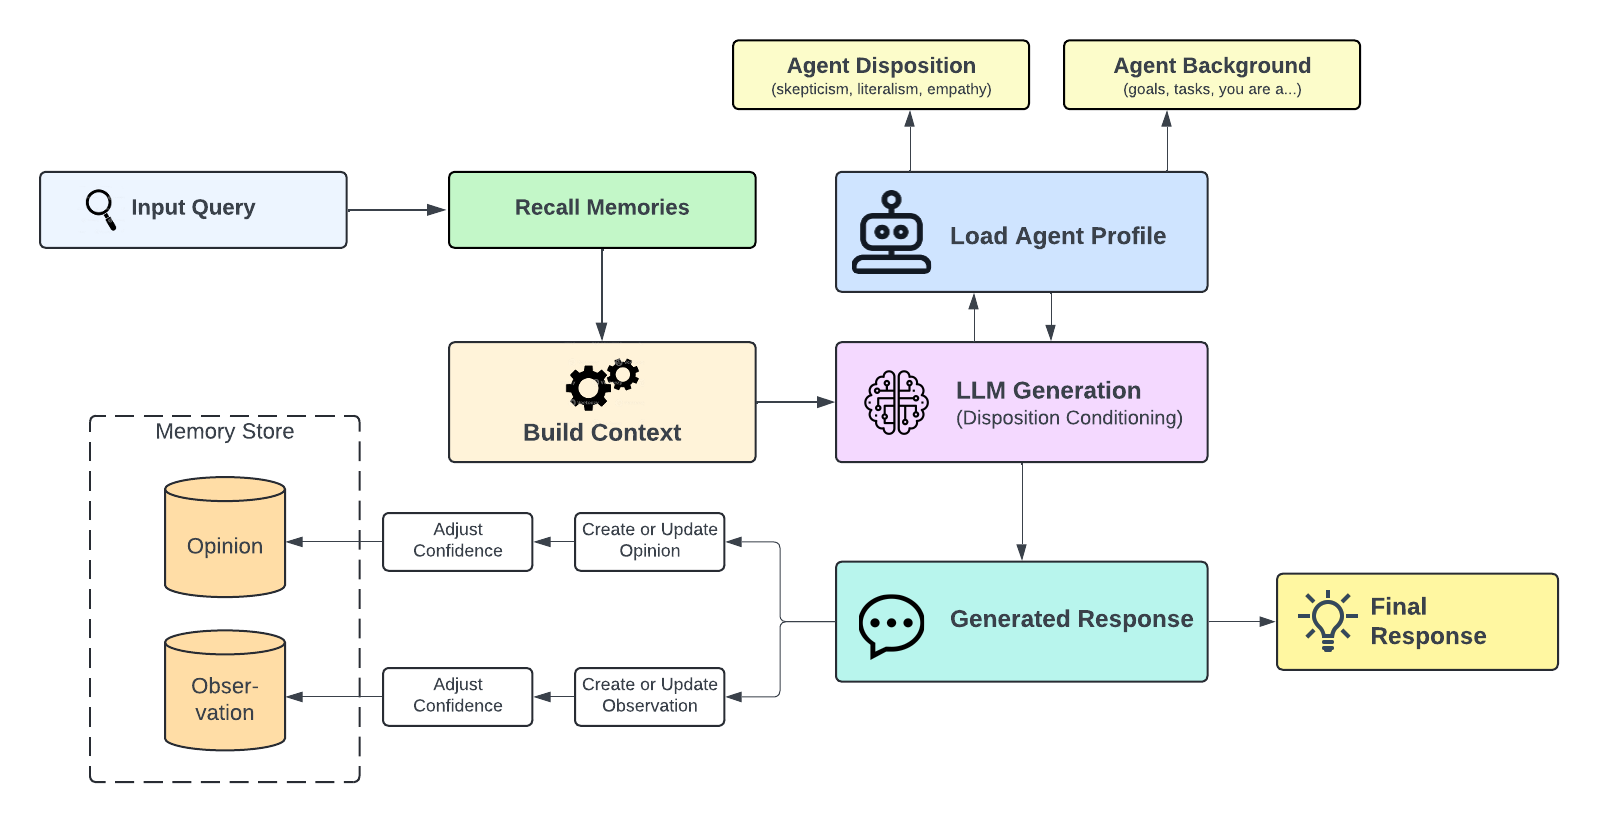
\includegraphics[width=\textwidth]{images/reflect-diagram.png}
    \caption{CARA's reflect loop. Given an input query, the agent recalls memories via TEMPR, builds context, loads the bank-specific profile (background and disposition), and performs disposition-conditioned generation, updating opinion and observation memories.}
    \label{fig:reflect-diagram}
\end{figure*}

The behavioral profile $\Theta$ and its bias-strength parameter $\beta$ determine how strongly this reflect step is encouraged to lean into the configured style. For low bias values ($\beta \approx 0$), system messages emphasize objectivity and downplay stylistic constraints. For intermediate values ($\beta \approx 0.5$), they balance factual neutrality with preference-conditioned behavior. For high bias values ($\beta \approx 1$), prompts explicitly encourage stronger, more opinionated language aligned with the specified preferences.

Each opinion formed in this way includes a confidence score $c \in [0,1]$, which we interpret as belief strength. Values near 1.0 indicate very strong conviction, mid-range values indicate moderate or tentative beliefs, and low values indicate weak, easily revisable views. This scalar makes it possible to track not only what the agent believes, but also how firmly it holds those beliefs, which is important when opinions are later reinforced or revised as new evidence arrives.

\begin{figure}[t]
\centering
\begin{tcolorbox}[
    colback=teal!5!white,
    colframe=teal!60!black,
    title={Trusting, Flexible, Empathetic Profile ($S=1, L=2, E=5$)},
    fonttitle=\bfseries,
    coltitle=white,
    colbacktitle=teal!60!black,
    boxrule=0.8pt,
    arc=1mm,
    enhanced,
    width=0.95\linewidth
]
\textbf{Opinion Formed:}

``Remote work is a net positive because it removes commute time and creates space for more flexible, self-directed work.''

\textbf{Emphasis:} Autonomy, flexibility, creative freedom
\end{tcolorbox}

\vspace{0.3cm}

\begin{tcolorbox}[
    colback=teal!5!white,
    colframe=teal!60!black,
    title={Skeptical, Literal, Detached Profile ($S=5, L=5, E=1$)},
    fonttitle=\bfseries,
    coltitle=white,
    colbacktitle=teal!60!black,
    boxrule=0.8pt,
    arc=1mm,
    enhanced,
    width=0.95\linewidth
]
\textbf{Opinion Formed:}

``Remote work risks undermining consistent performance because it makes it harder to maintain structure, oversight, and shared routines.''

\textbf{Emphasis:} Structure, accountability, consistency
\end{tcolorbox}

\caption{Example of preference-conditioned opinion formation. Two agents with opposite behavioral profiles access identical facts about remote work but form different opinions based on their configured disposition parameters.}
\label{fig:preference-conditioned-opinions}
\end{figure}


Figure~\ref{fig:preference-conditioned-opinions} illustrates how different behavioral profiles lead to systematically different opinions when presented with the same factual evidence.

\subsection{Opinion Reinforcement}

So far, we have described how CARA forms new opinions. In a long-lived system, those opinions should also be able to evolve as new information is retained.
When new facts arrive via TEMPR's retain pathway, CARA updates any related opinions in three steps:

\textbf{\textit{1) Identify Candidates.}} Use entity overlap and semantic similarity to find opinions that are plausibly related to the new facts. For each new fact $f$ with entities $\mathcal{E}_f$ and embedding $v_f$, we identify candidate opinions:
\begin{equation}
\mathcal{O}_{\text{cand}} = \{o \in \mathcal{O} : |\mathcal{E}_o \cap \mathcal{E}_f| > 0 \text{ or } \text{sim}(v_o, v_f) > \theta\}
\end{equation}
where $\text{sim}(v_o, v_f)$ is the cosine similarity between the opinion and fact embeddings, and $\theta$ is a similarity threshold.

\textbf{\textit{2) Assess the Evidence.}} For each candidate opinion $o \in \mathcal{O}_{\text{cand}}$, classify the relationship between the new facts and the current opinion. Let $\text{Assess}(o, f)$ be a function that returns one of $\{\text{reinforce}, \text{weaken}, \text{contradict}, \text{neutral}\}$ based on LLM analysis of the relationship.

\textbf{\textit{3) Apply an Update.}} Adjust the opinion's confidence score (and, for strong contradictions or refinements, optionally its text) according to the assessed relationship. Let $c$ be the current confidence and $c'$ be the updated confidence. The update rule is:
\begin{equation}
c' = \begin{cases}
\min(c + \alpha, 1.0) & \text{if Assess}(o, f) = \text{reinforce} \\
\max(c - \alpha, 0.0) & \text{if Assess}(o, f) = \text{weaken} \\
\max(c - 2\alpha, 0.0) & \text{if Assess}(o, f) = \text{contradict} \\
c & \text{if Assess}(o, f) = \text{neutral}
\end{cases}
\end{equation}
where $\alpha \in (0,1)$ is a step size parameter. For contradicting evidence, we may also update the opinion text $t$ to reflect the new nuance.

The update logic is designed to keep opinion trajectories stable but responsive. Small amounts of evidence lead to small changes, preventing opinions from oscillating in response to individual examples, while repeated reinforcement or strong contradictions can substantially shift the confidence. The behavioral profile can also influence how quickly opinions move (for example, a more cautious configuration may use a smaller $\alpha$), although we leave detailed exploration of such settings to future work.

Overall, reinforcement ensures that opinions reflect both the system's initial configuration (via the behavioral profile $\Theta$) and its subsequent evidence, rather than being fixed at creation time or overwritten wholesale when new information appears.

\subsection{Background Merging}

In addition to opinions, an agent's background description $h$ evolves as users provide more biographical information. If handled naively, this can quickly lead to contradictions or unwieldy, concatenated prompts.

Over time, new background snippets may complement existing information (e.g., adding work history where none existed), conflict with prior statements (e.g., ``born in Texas'' vs.\ ``born in Colorado''), or refine previous information (e.g., ``works in tech'' vs.\ ``works as a machine learning engineer at a startup'').

To keep the background coherent, CARA uses an LLM-powered merging procedure. Given the current background $h$ and a new snippet $h_{\text{new}}$, we prompt the model to produce a revised background $h'$ that \textbf{\textit{1)}} resolves direct conflicts in favor of the new information when appropriate, \textbf{\textit{2)}} appends non-conflicting details to enrich the description, \textbf{\textit{3)}} maintains a consistent first-person voice (``I'' rather than ``You''), and \textbf{\textit{4)}} remains concise (e.g., targeting a length under a few hundred characters).

Formally, the merging function is:
\begin{equation}
h' = \text{Merge}_{\text{LLM}}(h, h_{\text{new}})
\end{equation}

\begin{figure}[t]
\centering
\begin{tcolorbox}[
    colback=teal!5!white,
    colframe=teal!60!black,
    title=Background Merging Example,
    fonttitle=\bfseries,
    coltitle=white,
    colbacktitle=teal!60!black,
    boxrule=0.8pt,
    arc=1mm,
    enhanced,
    width=0.95\linewidth
]
\textbf{Current Background:}

``I was born in Colorado.''

\vspace{0.2cm}

\textbf{New Snippet:}

``You were born in Texas and have 10 years of startup experience.''

\vspace{0.2cm}

\textbf{Merged Background:}

``I was born in Texas and have 10 years of startup experience.''
\end{tcolorbox}

\caption{Example of background merging. The conflicting birthplace is resolved in favor of the new information, and the new work-history detail is added.}
\label{fig:background-merging}
\end{figure}

Figure~\ref{fig:background-merging} illustrates this process. As a preprocessing step, user-provided snippets are normalized into first person before merging, so that inputs such as ``You are a creative engineer'' become ``I am a creative engineer.'' This keeps the internal representation consistent with the way backgrounds are referenced in prompts. By maintaining a single, merged background per bank, CARA keeps identity information compact and coherent even as new biographical details accumulate over time.

\subsection{Preference-Conditioned Reasoning Examples}

We conclude this section with brief examples showing how CARA produces distinct and evolving viewpoints using the same underlying memory.

\subsubsection{Example: Opinion Evolution}

CARA's reinforcement mechanism also supports opinion change over time. Suppose a bank starts with the opinion:
\begin{equation}
o_0 = (\text{``Python is the best general-purpose language for data science''}, c_0 = 0.70, \tau_0)
\end{equation}

As new facts are retained via TEMPR, related evidence can strengthen or weaken this belief. For instance, a fact about Python's dominant ecosystem in AI/ML might lead to a modest increase in confidence:
\begin{equation}
o_1 = (\text{``Python is the best general-purpose language for data science''}, c_1 = 0.85, \tau_1)
\end{equation}

Later facts about performance advantages and growing adoption of alternatives (e.g., Julia or Rust in certain domains) might decrease confidence and encourage a more qualified opinion:
\begin{equation}
o_2 = (\text{``Python is strong for data science but has trade-offs''}, c_2 = 0.55, \tau_2)
\end{equation}

In this way, opinions become trajectories rather than static labels. They start from an initial, preference-conditioned formation step and are subsequently adjusted as new evidence accumulates.

Taken together, these mechanisms show how CARA turns the static memory structures provided by TEMPR into a configurable, preference-conditioned reasoning process. In Section~\ref{sec:hindsight-architecture}, we combine TEMPR and CARA into the unified \our architecture and examine the end-to-end properties and empirical behavior of the full system.
